\documentclass{article}
\usepackage[utf8]{inputenc}
\usepackage{enumitem}
\usepackage{graphicx}

\title{440 Assignment 1}
\author{Xiaowei Zhang, 204007085 \\ Xinyuan Chen, 197001668}
\date{November 2021}

\begin{document}
\maketitle

\section*{Problem 1}
(Lugoi, 244, 0, 244), (Mehadia, 311, 70, 241), (Lugoi, 384, 140, 244), (Drobeta, 387, 145, 242), (Craiova, 425, 265, 160), (Timisoara, 440, 111, 329), (Mehadia, 451, 210, 241), (Mehadia, 461, 220, 241), (Pitesti, 503, 403, 100), (Bucharest, 504, 504, 0)

\section*{Problem 2}
\begin{enumerate}[label=(\alph*)]

\item
Breadth first search: 1 \verb|->| 2 \verb|->| 3 \verb|->| 4 \verb|->| 5 \verb|->| 6 \verb|->| 7 \verb|->| 8 \verb|->| 9 \verb|->| 10 \verb|->| 11\\
Depth-limited search with limit 3: 1 \verb|->| 2 \verb|->| 4 \verb|->| 8 \verb|->| 9 \verb|->| 5 \verb|->| 10 \verb|->| 11\\
Iterative deepening search:\\
Limit = 0, 1\\
Limit = 1, 1 \verb|->| 2 \verb|->| 3\\
Limit = 2, 1 \verb|->| 2 \verb|->| 4 \verb|->| 5 \verb|->| 3 \verb|->| 6 \verb|->| 7\\
Limit = 3, 1 \verb|->| 2 \verb|->| 4 \verb|->| 8 \verb|->| 9 \verb|->| 5 \verb|->| 10 \verb|->| 11\\

\item
Bidirectional search works quite well on this problem.\\
Forward BFS: 1 \verb|->| 2 \verb|->| 3\\
Backward BFS: 11 \verb|->| 5 \verb|->| 2\\
They meet at 2. The branching factor of Forward BFS is 2 and the branching factor of Backward BFS is 1.


\end{enumerate}
\section*{Problem 3}
\begin{enumerate}[label=(\alph*)]
\item True, the only difference between BFS and uniform-cost search is that uniform-cost search expands the node with the lowest $g$ instead of of the shallowest node.
\item True.
\item True, the only difference between uniform-cost search and $A^*$ is that in $A^*$ search $f=g+h$ whereas in uniform-cost search $f=g$.
\item False, it just return the first path that contains the goal.
\item False, optimal only if all the costs of the edges are equal.
\item True.
\item True.
\item False.
\item True.
\end{enumerate}

\section*{Problem 4}
Advantage: The algorithm gives a search that is effectively breadth-first with the low memory requirements of depth-first search.\\
Disadvantage: Need time and wasted calculations at each iteration.

\section*{Problem 5}
Prove by induction: Suppose $h$ is a consistent heuristic function, $n$ is any node, $n'$ is any successor of $n$, $c(n,n')$ is the step cost of reaching $n'$ from $n$, so $h(n) \leq c(n,n')+h(n')$. We want to prove a consistent heuristic $h$ is also admissible, i.e. it never overestimates the cost of reaching the goal.\\
Base case: Let $n_1$ to be the predecessor of the goal node $n_0$, and $h(n_0)=0$. Since $h$ is consistent, $h(n_1) \leq c(n_1,n_0)+h(n_0) = c(n_1,n_0) + 0 = c(n_1,n_0)$, so it is bounded by the true cost and hence admissible.\\
Inductive step: Suppose $h$ is admissible for node $n_{i}$, $h(n_{i+1}) \leq c(n_{i+1},n_{i})+h(n_{i}) \leq c(n_{i+1},n_{i}) + c(n_{i},n_{i-1})+ h(n_{i-1}) \leq ... \leq c(n_{i+1},n_{i}) + c(n_{i},n_{i-1})+ ... + c(n_1,n_0) + h(n_0) \leq \sum_{j=1}^{i+1} c(n_j,n_{j-1})$, so it is bounded by the true cost and hence admissible.\\
Above all, if a heuristic function is consistent, it is also admissible.\\
Counter example see figure 1: from $x$ to $z$, $h(x) = 100 \leq 80+70=150$, $h(y) = 10 \leq 70$, so $h$ is admissible. However, $h(x) = 100 > h(y) + 80 = 90$, so $h$ is not consistent.
\begin{figure}
        \centering
        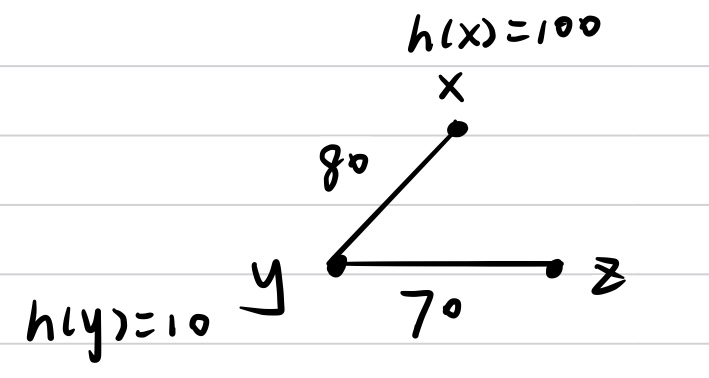
\includegraphics[width=0.6\textwidth]{5.jpg}
        \caption{Problem 5}
\end{figure}

\section*{Problem 6}
The variable that is most constrained means the variable can quickly fail. By choosing that, it can avoid pointless searches so as to save time and space.\\
The value that is least constraining means it the most likely to succeed. By choosing that, it can find the first solution quickly.

\section*{Problem 7}
\begin{enumerate}[label=(\alph*)]
\item The best move for the MAX player using the minimax procedure is C.
\item See figure 2.
\begin{figure}
        \centering
        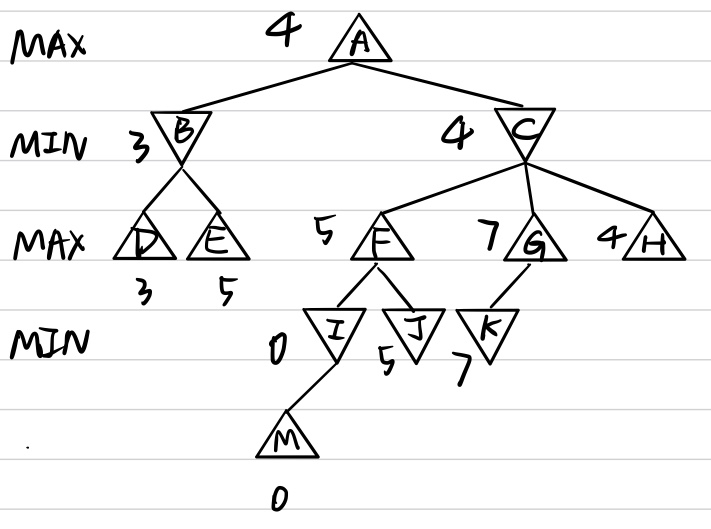
\includegraphics[width=0.6\textwidth]{7b.jpg}
        \caption{Problem 7(b)}
\end{figure}
\item See figure 3. 
\begin{figure}
        \centering
        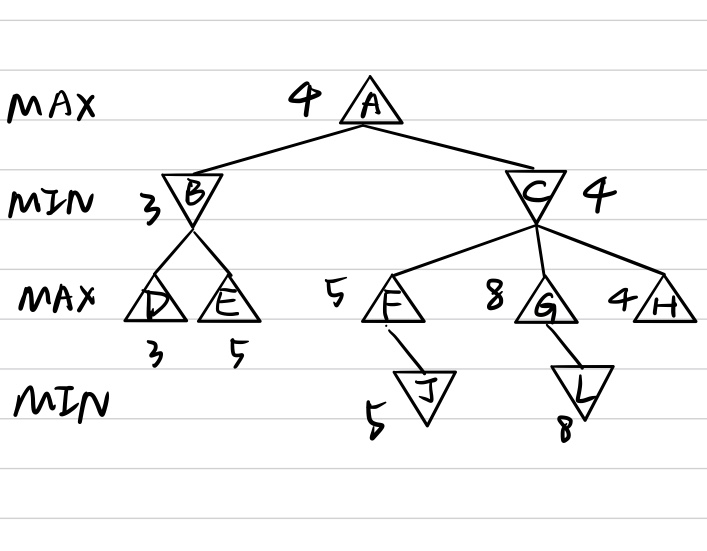
\includegraphics[width=0.6\textwidth]{7c.jpg}
        \caption{Problem 7(c)}
\end{figure}
Different pruning occurs because $\alpha$-$\beta$ pruning states that if $\alpha \geq \beta$, then the other branch will be pruned. From left to right, "the other branch" is right branch, whereas from right to left, "the other branch" is left branch. Also, depending on the order the pruning follows, alpha beta values change differently.
\end{enumerate}
\section*{Problem 8}
\begin{enumerate}[label=(\alph*)]
    \item $h(n)$ is both admissible and consistent.\\
    admissible: Since $h_1(n)\leq h^*(n)$, $h_2(n)\leq h^*(n)$, it is always true that $h(n)=min(h_1(n),h_2(n))=h_1(n)$ or $h_2(n)$, either one is smaller than $h^*(n)$, so $h(n)$ is admissible.\\
    consistent: Since $h_1(n) \leq c(n,n',a)+h(n')$, $h_2(n) \leq c(n,n',a)+h(n')$, it is always true that $min(h_1(n),h_2(n))$ is consistent.
    \item $h(n)$ is both admissible and consistent.\\
    admissible: Since $h_1(n)\leq h^*(n)$, $h_2(n)\leq h^*(n)$, $0<w<1$, $h(n)=wh_1(n)+(1-w)h_2(n)\leq wh^*(n) + (1-w)h^*(n) = h^*(n)$, so $h(n)$ is admissible.\\
    consistent: Since $h_1(n) \leq c(n,n',a)+h(n')$, $0<w<1$, $h_2(n) \leq c(n,n',a)+h(n')$, $h(n)=wh_1(n)+(1-w)h_2(n) \leq wc(n,n',a)+wh(n')+(1-w)c(n,n',a)+(1-w)h(n')= c(n,n',a)+h(n')$, so $h(n)$ is consistent.
    \item $h(n)$ is both admissible and consistent.\\
    admissible: Since $h_1(n)\leq h^*(n)$, $h_2(n)\leq h^*(n)$, it is always true that $h(n)=min(h_1(n),h_2(n))=h_1(n)$ or $h_2(n)$, either one is smaller than $h^*(n)$, so $h(n)$ is admissible.\\
    consistent: Since $h_1(n) \leq c(n,n',a)+h_1(n')$, $h_2(n) \leq c(n,n',a)+h_2(n')$, it is always true that $max(h_1(n),h_2(n))$ is consistent.\\
    We prefer to use $max(h_1(n),h_2(n))$ for $A^*$ because with greater h-value, we can expand less nodes and it means we are more close to the goal.
\end{enumerate}
\section*{Problem 9}
\begin{enumerate}[label=(\alph*)]
    \item For problems with no local maximums.
    \item For problems with only plateaus.
    \item For problems with both local maximums and plateaus.
    \item Since we know the value of each state we visit, we keep running values for max and only update when we find a larger one. Return the state with the largest value.
    \item keep track of all states that have been traversed and whenever current state is in tracked states, halt and restart. Don't randomly pick start point. Pick those states that are not in the tracked list.
    \item After adapting randomness to gradient ascent search, if current gradient is 0, then the probability of choosing other states is positively proportional to the temperature, otherwise, the probability is negatively proportional to the temperature and positively proportional to the absolute value of the gradient.
\end{enumerate}
\end{document}


